\chapter{Validation of the Proposed Method}
\label{ch:validation}
 
\section{Approach}
\label{sec:valapproach}
 
The formulation of Chapter~\ref{ch:method} is assessed in two stages, which
answer different questions and are kept separate throughout.
 
\emph{Verification} asks whether the implementation solves the equations it is
intended to solve. It is carried out in Section~\ref{sec:nemes} by reproducing
the benchmark of \textcite{nemesModelingCylindricalAdhesively2009}, the source
of the variational procedure itself: the same geometry, the same material
properties and the same loading configuration are supplied to the present code,
and the resulting stress distributions are compared with those published. Since
both are analytical solutions of the same boundary value problem, agreement
tests the implementation and nothing else; disagreement would indicate an error
in the coding of the energy integrals, the boundary conditions or the closure
for $\alpha_1$, rather than a deficiency of the model.
 
Two benchmarks are used, chosen so that between them they exercise every
branch of the formulation: \textcite{nemesModelingCylindricalAdhesively2009}
in Section~\ref{sec:nemes} and \textcite{hassaniehGluedinrodTimberJoints2018} in
Section~\ref{sec:hassanieh}. Section~\ref{sec:valsynthesis} sets out what the
two together establish.
 
\emph{Validation} asks whether the equations describe reality, and requires
measured data. It is carried out in Chapter 8 against the database of bond
tests assembled from the literature.
 
\newpage
\section[Verification against Nemes and Lachaud (2009)]{Verification against Nemes and Lachaud\\(2009)}
\label{sec:nemes}
 
\subsection{Benchmark configuration}
\label{sec:nemescase}
 
\textcite{nemesModelingCylindricalAdhesively2009} analyse a tubular adhesive
joint loaded in tension at both ends, which in the terminology of
Section~\ref{sec:test} is the \emph{pull--pull} configuration (shown in Figure~\ref{fig:nemestest}). 
\begin{figure}[H]
\centering
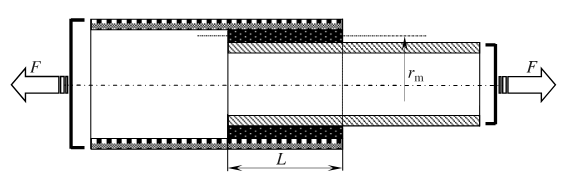
\includegraphics[width=0.8\linewidth]{nemes test.png}
\caption{Diagram of the adhesively bonded joint from \textcite{nemesModelingCylindricalAdhesively2009}.}
\label{fig:nemestest}
\end{figure}
The three concentric layers of their assembly map directly onto those of
Section~\ref{sec:scope}: the inner aluminium tube takes the place of the bar,
the adhesive layer that of the rib layer, and the outer carbon/epoxy tube that
of the concrete. The geometry and material properties are those of their
Table~2 and are reproduced in Table~\ref{tab:nemesparams}.
 
\begin{table}[htbp]
\centering
\caption{Benchmark parameters, after Table~2 of
         \textcite{nemesModelingCylindricalAdhesively2009}.}
\label{tab:nemesparams}
\begin{tabular}{@{}cccc@{}}
\hline
 & Inner tube & Adhesive & Outer tube \\
 & \shortstack[c]{Aluminium\\ALU 7075} & \shortstack[c]{Araldite Redux\\340\,SP} & \shortstack[c]{Carbon/epoxy\\G0969/M18} \\
\hline
Inner radius (mm)  & $r_i = 44.8$   & $r_{ic} = 47.8$ & $r_{ec} = 48.0$ \\
Outer radius (mm)  & $r_{ic} = 47.8$ & $r_{ec} = 48.0$ & $r_e = 50.0$ \\
$E$ (MPa)          & 72\,000        & 2\,700          & 44\,080 \\
$G$ (MPa)          & 27\,692        & 1\,000          & 16\,640 \\
$\nu$              & 0.30           & 0.35            & 0.325 \\
\hline
\multicolumn{4}{@{}p{\linewidth}@{}}{\raggedright Overlap length $L = \SI{50}{\milli\metre}$;\quad
                   applied stress $f = \SI{100}{\mega\pascal}$ on the inner
                   tube} \\
\hline
\end{tabular}
\end{table}
 
Two features of the benchmark make it a searching test of the implementation.
The adherends are stiff relative to a very thin and very compliant interlayer,
$r_{ec} - r_{ic} = \SI{0.2}{\milli\metre}$ with $E_c/E_1 = 0.0375$, so the
shear-lag behaviour is pronounced; and the inner tube is hollow,
$r_i \ne 0$, which exercises the general form of the radial integrals rather
than the solid-bar limit used throughout Chapter~\ref{ch:method}. The outer
tube is quoted as orthotropic, but the values given satisfy
$G_{xy} = E_x/[2(1+\nu_{xy})]$ to within \SI{0.04}{\percent}, so the layer is
isotropic for the purposes of this calculation and the isotropic form of the
energy density of Section~\ref{sec:energy} applies without modification.
 
No parameter was adjusted or calibrated. The code of
Chapter~\ref{ch:method} was run with \texttt{setup = 'pull-pull'} and the
values of Table~\ref{tab:nemesparams} substituted directly.
 
\subsection{Shear stress distribution}
\label{sec:nemesshear}
 
Figure~\ref{fig:nemesshear} compares the computed interfacial shear stress
with Figure~3(b) of \textcite{nemesModelingCylindricalAdhesively2009}. The
agreement is close in every respect that characterises the distribution.
 
\begin{figure}[H]
\centering
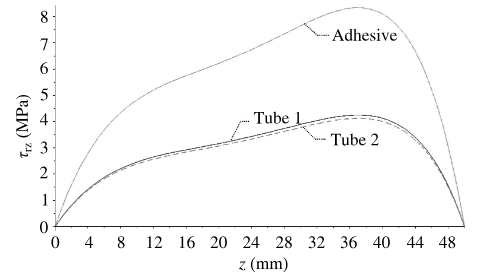
\includegraphics[width=0.7\linewidth]{nemes shear.png}\\[1.5mm]
{\small (a)}\\[5mm]
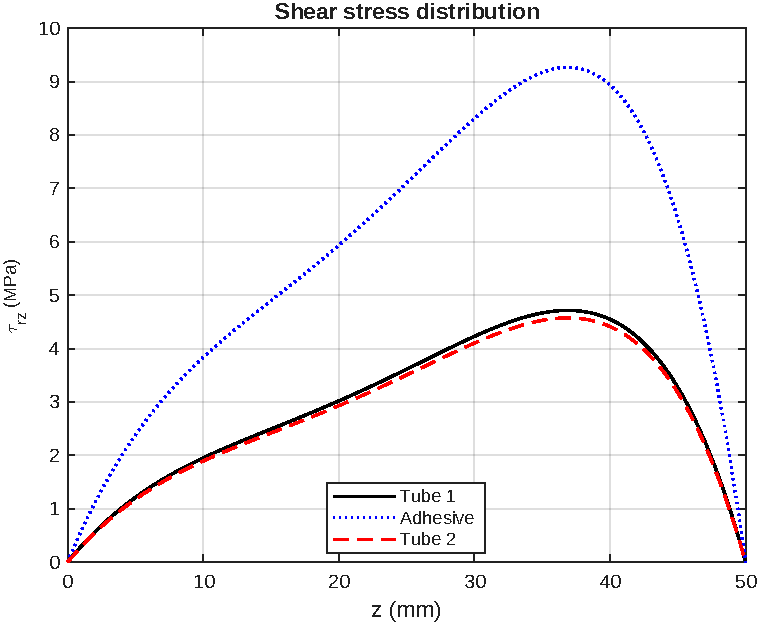
\includegraphics[width=0.7\linewidth]{shear nemes validation.pdf}\\[1.5mm]
{\small (b)}
\caption[Interfacial shear stress: benchmark and present model]{Interfacial
         shear stress along the joint. (a)~Figure~3(b) of
         \textcite{nemesModelingCylindricalAdhesively2009}; (b)~the present
         model, run with the parameters of Table~\ref{tab:nemesparams} and no
         adjustment.}
\label{fig:nemesshear}
\end{figure}
 
\begin{table}[htbp]
\centering
\caption{Shear stress $\tau_{rz}$ at the benchmark load, present model against
         Figure~3(b) of \textcite{nemesModelingCylindricalAdhesively2009}.
         Tube values are taken at the mid-thickness of the layer, the adhesive
         value at the interface.}
\label{tab:nemesshear}
\begin{tabular}{@{}l c p{0.28\linewidth} c@{}}
\hline
 & Present model & \raggedright\textcite{nemesModelingCylindricalAdhesively2009}
 & Difference \\
\hline
Peak $\tau_{rz}$, inner tube (MPa)  & 4.72  & $\approx 4.25$ & $+11\%$ \\
Peak $\tau_{rz}$, adhesive (MPa)    & 9.26  & $\approx 8.4$  & $+10\%$ \\
Peak $\tau_{rz}$, outer tube (MPa)  & 4.57  & $\approx 4.1$  & $+12\%$ \\
Location of peak, $z$ (mm)          & 36.9  & $\approx 37$   & --- \\
Ratio adhesive\,/\,inner tube       & 1.97  & $\approx 1.98$ & $-0.6\%$ \\
\hline
\end{tabular}
\end{table}
 
The computed distribution vanishes at both free ends, as required by
\eqref{eq:bcshear}; rises steeply from the unloaded end; and peaks at
$z = \SI{36.9}{\milli\metre}$, against approximately \SI{37}{\milli\metre}
read from the published figure. The marked asymmetry of the distribution,
which is the distinguishing feature of the model that retains $\sigma_{rr}$ ---
Figure~3(a) of the same work, computed with $\sigma_{rr} = 0$, is nearly
symmetric with a broad plateau --- is reproduced. The ratio of the adhesive
peak to the adherend peak, 1.97 against 1.98, is matched to better than one
per cent, which is a stringent test because that ratio is fixed by the radial
distribution of $\tau_{rz}$ through \eqref{eq:bar}--\eqref{eq:conc} and is
independent of the magnitude of the solution.
 
The absolute magnitudes are uniformly about ten per cent higher than the
published values. The uniformity is the significant observation: all three
curves are scaled by the same factor, to within the precision with which the
figures can be read, so the difference is a single multiplicative factor on
$\mathrm{d}\sigma_z^{s}/\mathrm{d}z$ rather than a distortion of the solution.
A structural error --- a mis-stated boundary condition, a missing term in the
energy, an incorrect closure for $\alpha_1$ --- would alter the shape, the
peak location or the inter-layer ratios, and none of these is affected.

\newpage
\subsection{Circumferential stress distribution}
\label{sec:nemeshoop}
 
The comparison of hoop stress with Figure~4(b) of
\textcite{nemesModelingCylindricalAdhesively2009}, shown in
Figure~\ref{fig:nemeshoop} and tabulated in Table~\ref{tab:nemeshoop}, is
less conclusive, for a reason that is a property of the quantity rather than
of either calculation.
 
\begin{figure}[H]
\centering
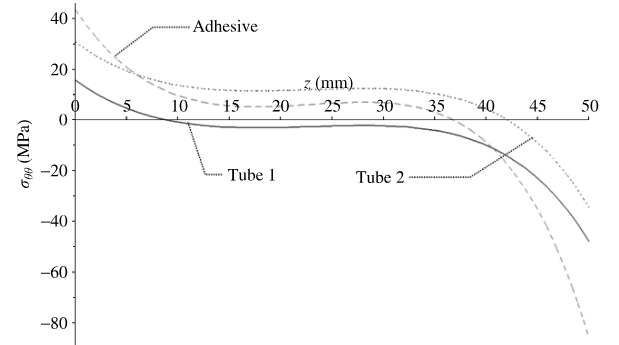
\includegraphics[width=0.72\linewidth]{nemes hoop.png}\\[1.5mm]
{\small (a)}\\[5mm]
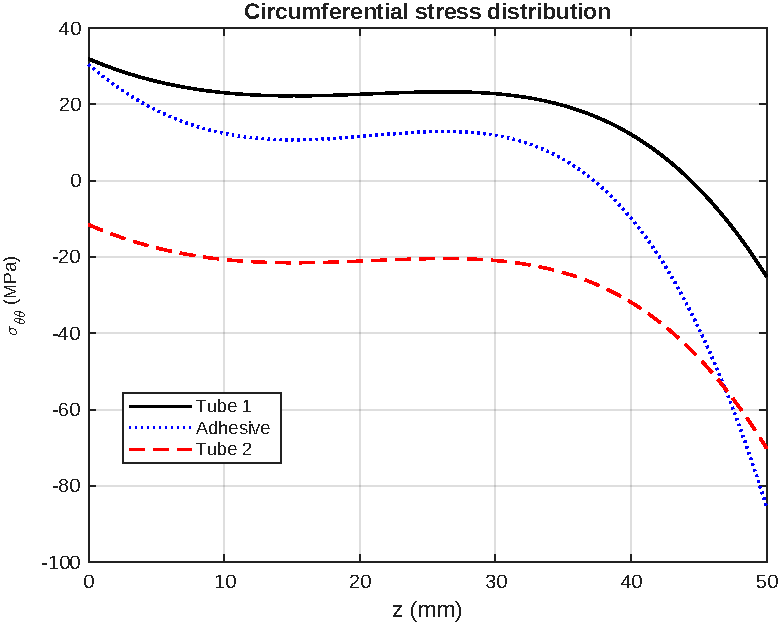
\includegraphics[width=0.72\linewidth]{hoop nemes validation}\\[1.5mm]
{\small (b)}
\caption[Circumferential stress: benchmark and present model]{Circumferential
         stress along the joint. (a)~Figure~4(b) of
         \textcite{nemesModelingCylindricalAdhesively2009}; (b)~the present
         model, run with the parameters of Table~\ref{tab:nemesparams} and no
         adjustment.}
\label{fig:nemeshoop}
\end{figure}

\newpage
In the adhesive the agreement is good: the computed value at the loaded end is
\SI{30.5}{\mega\pascal} against approximately \SI{30}{\mega\pascal}, and the
interior plateau is \SI{12.8}{\mega\pascal} against approximately
\SI{11}{\mega\pascal}. The adhesive is the one layer for which the comparison
is unambiguous, because $\sigma_\theta^{r}$ of \eqref{eq:rib} is independent
of $r$ and the thinness of the layer therefore removes any question of where
the value is taken.
 
\begin{table}[htbp]
\centering
\caption{Circumferential stress $\sigma_\theta$ at the benchmark load, present
         model against Figure~4(b) of
         \textcite{nemesModelingCylindricalAdhesively2009}. Tube values are
         taken at the mid-thickness of the layer, the adhesive value at the
         interface.}
\label{tab:nemeshoop}
\small
\begin{tabular*}{\linewidth}{@{\extracolsep{\fill}}lccc@{}}
\hline
$\sigma_\theta$ (MPa) & Present model
 & \textcite{nemesModelingCylindricalAdhesively2009} & Difference \\
\hline
Adhesive at $z = 0$           & $+30.5$ & $\approx +30$ & $+2\%$ \\
Adhesive, interior plateau    & $+12.8$ & $\approx +11$ & $+17\%$ \\
Inner tube at $z = 0$         & $+32.0$ & $\approx +15$ & $^{\dagger}$ \\
Outer tube at $z = 0$         & $-11.5$ & $\approx +41$ & $^{\dagger}$ \\
Inner tube, across the wall   & $+16.4$ to $+48.0$ & not stated & --- \\
\hline
\multicolumn{4}{@{}p{0.95\linewidth}@{}}{\raggedright $^{\dagger}$~Not
   comparable: the radius at which the published adherend curves are
   evaluated is not stated, and the computed value varies by a factor of
   three across the wall of the inner tube.} \\
\hline
\end{tabular*}
\end{table}
 
In the two adherends the computed curves differ from the published ones in
magnitude and, over part of the range, in sign. The hoop stress in those
layers is dominated by the term linear in $\alpha_1$ of \eqref{eq:bar} and
\eqref{eq:conc}, which varies strongly across the thickness: in the inner tube
the computed value at the loaded end ranges from \SI{16.4}{\mega\pascal} on
the bore to \SI{48.0}{\mega\pascal} at the adhesive interface, a factor of
three across \SI{3}{\milli\metre} of wall. The published figure does not state
the radius at which each curve is evaluated, so the two sets of curves are not
necessarily being compared at the same point. Given that sensitivity, the
difference in the adherend hoop stresses cannot be attributed to the
implementation on the available evidence, and no claim is made here either
way.
 
\subsection{Discussion}
\label{sec:nemesdiscussion}
 
Two observations follow.
 
The model reproduces the benchmark in every feature that is
independent of absolute scale: the shape of the shear distribution, its
asymmetry, the vanishing of the interfacial shear at both ends, the location
of the peak to within \SI{0.1}{\milli\metre}, and the ratio of adhesive to
adherend shear to better than one per cent. These are the features that test
the energy integration, the boundary conditions and the determination of
$\alpha_1$, and they are reproduced without adjustment.
 
The residual difference in magnitude, uniformly of order ten per cent, is
consistent with a difference in the treatment of a single scalar rather than
with an error in the formulation. Several possible explanations cannot be separated on the
available information: the published figures may have been produced with a
slightly different value of the applied stress or of one elastic constant than
appears in their Table~2; the radii at which the curves are plotted are not
stated; and the figures themselves can be read only to perhaps five per cent.
It is noted that \textcite{nemesModelingCylindricalAdhesively2009} report in
their conclusions a peak adhesive shear of approximately eight per cent of the
applied load, consistent with their Figure~3(b), against \SI{9.3}{\percent}
here.
 
The most significant of these is that
\textcite{nemesModelingCylindricalAdhesively2009} state the governing
differential equation but not its solution. Neither the general form adopted,
nor the constants of integration, nor the manner in which the four boundary
conditions were imposed is given, so the step from the fourth-order equation
to the plotted curves had to be reconstructed here and cannot be checked
against the source. That step is also the natural place for a uniform
difference to arise. It fixes the magnitude of $\sigma_z^{s}$ and hence of
every stress derived from it, whereas the shape of the distribution and the
ratios between the layers are fixed by the assumed stress field and are
insensitive to it. A difference confined to the solution of the governing
equation would therefore scale all three curves by the same factor and leave
the peak location unmoved, which is what is observed.
 
On this evidence the implementation is taken to be a correct realisation of
the variational formulation, and is carried forward to the concrete
application of Chapter~\ref{ch:method} with the configuration switched to
pull--push.
 
\section{Verification against Hassanieh et al. (2018)}
\label{sec:hassanieh}
 
\subsection{Rationale for a second benchmark}
\label{sec:whysecond}
 
Section~\ref{sec:nemes} establishes that the implementation reproduces the
formulation it was built from. That is a necessary check but a narrow one: a
single benchmark can be matched by a code that happens to be correct only for
the particular combination of geometry, material symmetry and root type that
the benchmark contains. A second, independent benchmark was therefore
selected to exercise the parts of the formulation that
\textcite{nemesModelingCylindricalAdhesively2009} does not.
 
textcite{hassaniehGluedinrodTimberJoints2018} analyse glued-in rod timber joints
using the same variational framework but with three substantive differences,
each of which tests a different part of the implementation:
 
\begin{itemize}
\item \emph{Their stress field is simpler.} They take the radial and
      tangential stresses to be equal, $\sigma_r = \sigma_\theta$, and obtain
      both from radial equilibrium instead of assuming a form for them. Their
      model therefore has no radial-stress parameter $\alpha_1$, and no second
      minimisation to determine it, as Section~\ref{sec:alpha} does here: the
      whole field follows from $\sigma_z^{s}$ alone. Reproducing their results
      therefore exercises the energy integration and the solution of the
      governing equation on their own, apart from the $\alpha_1$ machinery
      that the first benchmark tests.
\item \emph{Their rod is solid rather than hollow,} $r_i = 0$. The inner
      adherend of \textcite{nemesModelingCylindricalAdhesively2009} is a tube,
      so its radial integrals never reach the axis. A solid rod is what
      Chapter~\ref{ch:method} assumes throughout, so this benchmark tests the
      geometry the thesis model actually uses.
\item \emph{Their outer adherend is directional.} Timber is transversely
      isotropic: it has one stiffness along the grain and a much lower one
      across it. Both of Nemes and Lachaud's adherends are isotropic, with the
      same stiffness in every direction, so this is the only benchmark that
      tests the code on a material whose properties depend on direction.
\end{itemize}
 
A further advantage is that
\textcite{hassaniehGluedinrodTimberJoints2018} publish the coefficients of their
energy functional in closed form. The present code obtains those coefficients
by integrating the strain energy across the three layers symbolically,
so the published expressions provide a direct check on that integration,
independent of any comparison of plotted curves.
 
\subsection{Benchmark configuration}
\label{sec:hasscase}
 
The case selected is that of their Figure~4: a \SI{12}{\milli\metre} steel rod
glued into glulam over an embedment length of \SI{360}{\milli\metre} and
loaded in pull--pull to \SI{28.8}{\kilo\newton}, forty per cent of the
measured ultimate capacity. Parameters are given in
Table~\ref{tab:hassparams}.
 
\begin{table}[htbp]
\centering
\caption{Benchmark parameters, after
         \textcite{hassaniehGluedinrodTimberJoints2018}. Quantities marked
         $^{\dagger}$ are not stated in the source and are assumed.}
\label{tab:hassparams}
\begin{tabular}{llll}
\hline
 & Rod & Adhesive & Timber (glulam) \\
\hline
Inner radius (mm)   & $0$          & $a = 6$    & $b = 7$ \\
Outer radius (mm)   & $a = 6$      & $b = 7$    & $c = 60$ \\
$E$ (MPa)           & $200\,000^{\dagger}$ & $3\,000$ & $E_1 = 13\,000$,\ \ $E_2 = E_1/30$ \\
$G$ (MPa)           & ---          & ---        & $G = E_1/16$ \\
$\nu$               & $0.30^{\dagger}$ & $0.20$ & $\nu_{12} = \nu_{13} = 0.30^{\dagger}$ \\
\hline
\multicolumn{4}{l}{Embedment $L = \SI{360}{\milli\metre}$;\quad
                   $F = \SI{28.8}{\kilo\newton}$, hence
                   $f = F/\pi a^2 = \SI{254.6}{\mega\pascal}$} \\
\hline
\end{tabular}
\end{table}
 
The hole is \SI{2}{\milli\metre} oversize, giving a \SI{1}{\milli\metre} glue
line, and the half-width of the glulam for a \SI{12}{\milli\metre} rod is
\SI{60}{\milli\metre}. As in Section~\ref{sec:nemes}, no parameter was
adjusted.
 
\subsection{Results}
\label{sec:hassresults}
 
The roots of the characteristic equation come out real and distinct,
\begin{equation}
\label{eq:hassroots}
w_1 = \SI{0.0637}{\per\milli\metre}, \qquad
w_2 = \SI{0.0136}{\per\milli\metre},
\end{equation}
so the stress decays away from each end over characteristic lengths of
$1/w_1 = \SI{15.7}{\milli\metre}$ and $1/w_2 = \SI{73.6}{\milli\metre}$.
 
This is a second respect in which the benchmark complements the first. The
roots of Section~\ref{sec:nemes} are a complex conjugate pair, which makes
the stress oscillate as it decays; these are real, which makes it decay
smoothly without oscillation. Which of the two occurs depends on the sign of
the discriminant in \eqref{eq:roots}, and the solution is written
differently in each case, so between them the two benchmarks test both.
 
Three of the checks that follow need no reading of a published figure at
all, and so carry more weight than any curve comparison.
 
\paragraph{Interface continuity.} The radial and shear tractions are
continuous across both interfaces, $r = a$ and $r = b$. The difference is
exactly zero, not merely small, confirming that the assumed stress field has
been written and substituted correctly.
 
\paragraph{Energy coefficients.}
\textcite{hassaniehGluedinrodTimberJoints2018} publish two of their energy
coefficients as algebraic expressions,
$A = \tfrac{1}{2}a^2/E^{(1)} - \tfrac{1}{2}a^4/[E_1^{(2)}(b^2-c^2)]$ and
$D = a^4 f/[E_1^{(2)}(b^2-c^2)]$. The present code arrives at the same two
numbers by integrating the complementary energy symbolically, without using
their expressions:
\begin{equation}
\label{eq:hasscoeff}
A = \num{1.04037e-4}, \qquad
D = \num{-7.1491e-3},
\end{equation}
each agreeing with the published closed form to a ratio of $1.000000$. This
is the strongest single check in either benchmark, because it compares two
numbers directly rather than two curves read off a figure, and because it
tests the radial integration on its own.
 
\paragraph{Boundary conditions.} The rod carries no axial stress at the free
end and the full applied stress at the loaded end:
\SI{0.00}{\mega\pascal} at $z = 0$ and \SI{254.65}{\mega\pascal} at
$z = L$, against the imposed $f = \SI{254.6}{\mega\pascal}$. The
distribution between those two values is compared with their Figure~4(a) in
Figure~\ref{fig:hassaxial}.
 
The stress distributions themselves are compared with Figure~4 of the source
in Table~\ref{tab:hassresults} and Figures~\ref{fig:hassaxial}
to~\ref{fig:hasshoop}.
 
\begin{table}[htbp]
\centering
\caption{Present code against Figure~4 of
         \textcite{hassaniehGluedinrodTimberJoints2018}, evaluated on the glue
         line.}
\label{tab:hassresults}
\small
\begin{tabular}{@{}p{0.25\linewidth}r p{0.38\linewidth}r@{}}
\hline
 & Present code & \textcite{hassaniehGluedinrodTimberJoints2018} & Difference \\
\hline
$\sigma_z$ in the rod at $z = L$ (MPa) & 254.65 & 254.6 & $0.0\%$ \\
Peak $\tau_{rz}$ (MPa)                 & 5.09   & $\approx 4.8$  & $+6\%$ \\
\raggedright Location of peak, $z$ (mm) & 329    & $\approx 340$  & $-3\%$ \\
$\sigma_\theta$ at $z = 0$ (MPa)       & $+1.03$& $\approx +1$   & --- \\
$\sigma_\theta$ at $z = L$ (MPa)       & $-5.78$& $\approx -4.5$ & $+28\%$ \\
\raggedright Joint stiffness $K_s$ (kN/mm) & 201.0 & 112.7 & $+78\%$ \\
\hline
\end{tabular}
\end{table}
 
\begin{figure}[H]
\centering
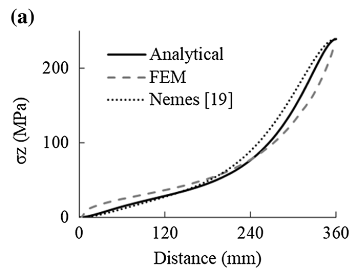
\includegraphics[width=0.70\linewidth]{hassanieh_fig4a.png}\\[1.5mm]
{\small (a)}\\[5mm]
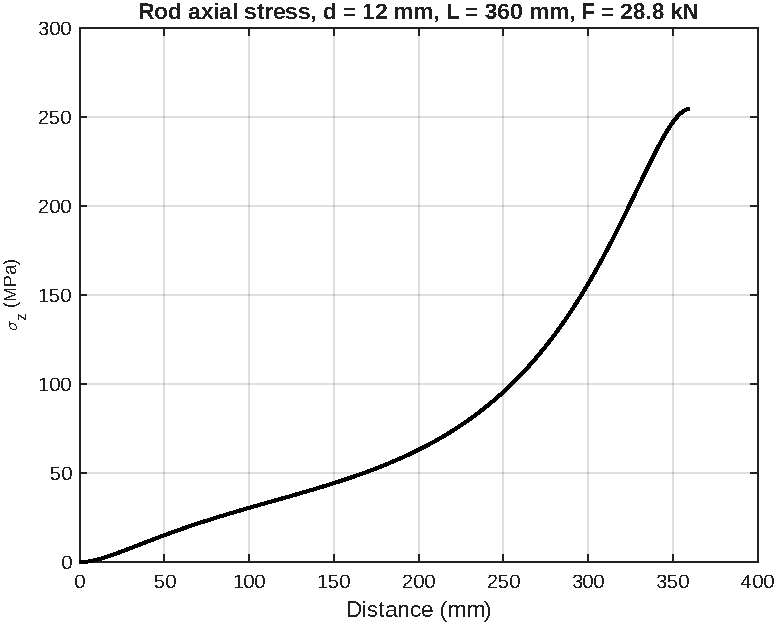
\includegraphics[width=0.70\linewidth]{hassanieh stress valid.pdf}\\[1.5mm]
{\small (b)}
\caption[Rod axial stress: benchmark and present model]{Axial stress in the
         rod along the embedment. (a)~Figure~4(a) of
         \textcite{hassaniehGluedinrodTimberJoints2018}; (b)~the present
         model. The stress rises from zero at the free end to the full
         applied \SI{254.6}{\mega\pascal} at the loaded end, slowly over the
         first half of the embedment and steeply over the last quarter. That
         shape is the load transfer concentrating near the loaded end, and it
         is what the shear distribution of Figure~\ref{fig:hassshear}
         differentiates.}
\label{fig:hassaxial}
\end{figure}
 
\begin{figure}[H]
\centering
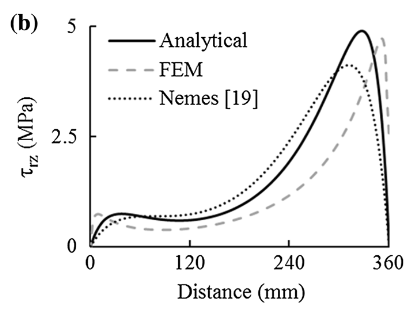
\includegraphics[width=0.70\linewidth]{hassanieh_fig4b.png}\\[1.5mm]
{\small (a)}\\[5mm]
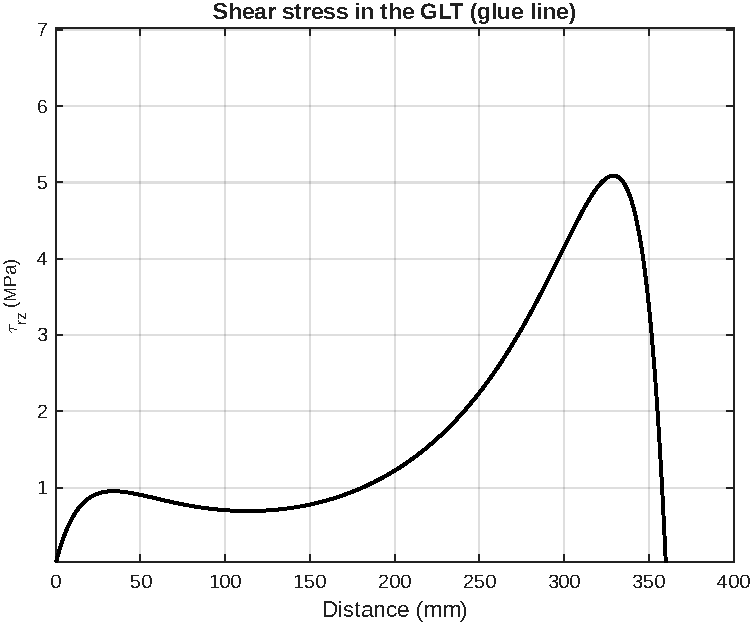
\includegraphics[width=0.70\linewidth]{hassanieh shear valid.pdf}\\[1.5mm]
{\small (b)}
\caption[Glue-line shear stress: benchmark and present model]{Shear stress on
         the glue line. (a)~Figure~4(b) of
         \textcite{hassaniehGluedinrodTimberJoints2018}; (b)~the present
         model, run with the parameters of Table~\ref{tab:hassparams} and no
         adjustment. Both show the same three-part profile: a local maximum
         about \SI{30}{\milli\metre} from the free end, a shallow trough
         through the middle of the bond line, and the true peak close to the
         loaded end. Comparison is with their analytical curve; the finite
         element and Nemes curves on their figure are shown for their own
         purposes.}
\label{fig:hassshear}
\end{figure}
 
\begin{figure}[H]
\centering
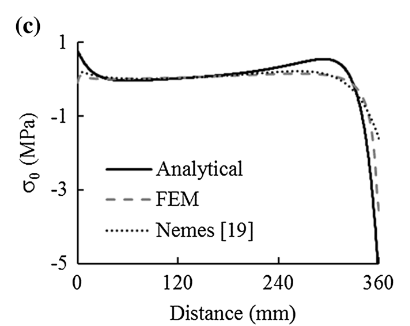
\includegraphics[width=0.70\linewidth]{hassanieh_fig4c.png}\\[1.5mm]
{\small (a)}\\[5mm]
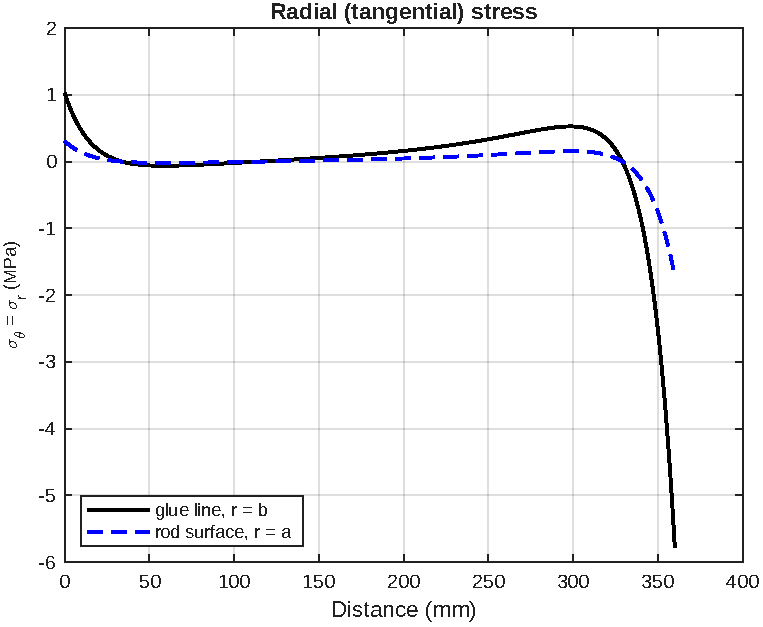
\includegraphics[width=0.70\linewidth]{hassanieh hoop valid.pdf}\\[1.5mm]
{\small (b)}
\caption[Tangential stress: benchmark and present model]{Tangential stress
         along the embedment, equal to the radial stress under the assumption
         of \textcite{hassaniehGluedinrodTimberJoints2018}. (a)~Their
         Figure~4(c); (b)~the present model. The stress is tensile at the free
         end, passes through a near-zero plateau, recovers to a small
         positive value near $z = \SI{300}{\milli\metre}$ and then turns
         sharply compressive over the last tenth of the embedment. Panel~(b)
         is drawn at two radii, the glue line $r = b$ and the rod surface
         $r = a$, which the single published curve does not distinguish; the
         two coincide over most of the length and separate only where the
         stress is changing fastest.}
\label{fig:hasshoop}
\end{figure}
 
\begin{figure}[H]
\centering
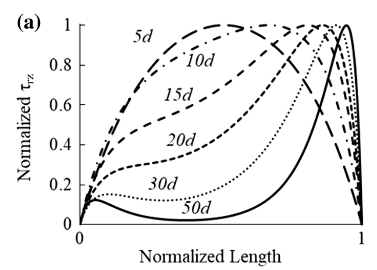
\includegraphics[width=0.70\linewidth]{hassanieh_fig8a.png}\\[1.5mm]
{\small (a)}\\[5mm]
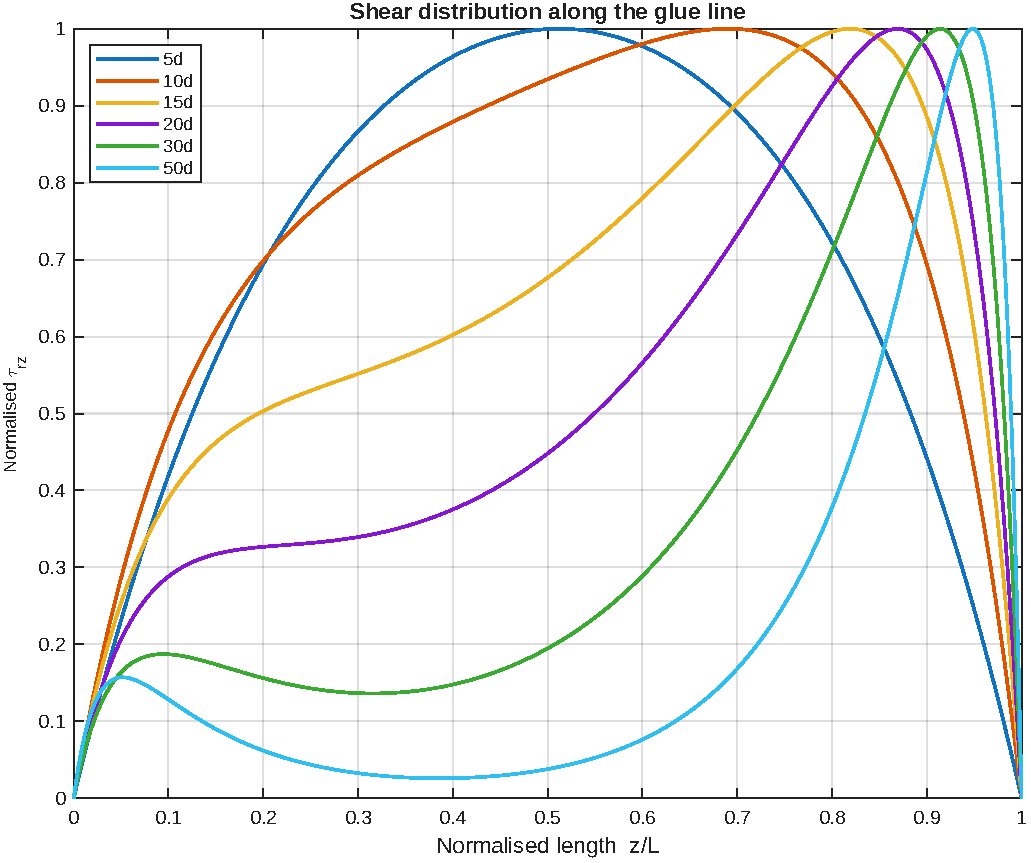
\includegraphics[width=0.70\linewidth]{hassanieh norm length.pdf}\\[1.5mm]
{\small (b)}
\caption[Shear distribution against embedment length]{Normalised shear
         distribution along the glue line for embedment lengths from
         $L/d = 5$ to $50$, each curve scaled to its own maximum.
         (a)~Figure~8(a) of
         \textcite{hassaniehGluedinrodTimberJoints2018}; (b)~the present
         model. At $L/d = 5$ the peak lies near mid-length; as the embedment
         lengthens it migrates to the loaded end and a trough opens up over
         the middle of the joint, until at $L/d = 50$ the interior carries
         almost no shear at all. This comparison is of a trend across six
         embedment lengths rather than of a single curve.}
\label{fig:hassld}
\end{figure}

\newpage
Both distributions come out the right shape. The shear stress
(Figure~\ref{fig:hassshear}) rises from zero at the free end to a small local
maximum near $z = \SI{30}{\milli\metre}$, drops back to a shallow trough
around mid-length, then climbs to its true peak close to the loaded end and
returns to zero there. Their Figure~4(b) shows the same three stages in the
same places. The tangential stress (Figure~\ref{fig:hasshoop}) is tensile at
the free end, stays close to zero through the middle, and turns sharply
compressive over the last tenth of the embedment, as in their Figure~4(c).
 
Neither shape is arbitrary. In a joint this long the load is transferred
almost entirely within a short distance of each end, so the middle of the
bond line carries very little. That is what produces both the trough in the
shear and the compression at the loaded end.
 
The model also reproduces how the distribution changes as the embedment gets
longer. This is a harder test, because it compares a trend rather than a
single curve. Figure~\ref{fig:hassld} repeats the calculation for $L/d$ from
$5$ to $50$ alongside their Figure~8(a). At $L/d = 5$ the shear peaks at
mid-length. As the embedment lengthens the peak moves towards the loaded end
and the middle of the joint carries less and less, until at $L/d = 50$ the
shear there is only three per cent of its peak. The roots in
\eqref{eq:hassroots} explain why: the stress decays over a length of about
$1/w_2 = \SI{73.6}{\milli\metre}$, so once the embedment is several times
that, the two ends no longer influence one another.
 
\subsection{Discussion}
\label{sec:hassdiscussion}
 
Agreement on the stress field is good; agreement on the stiffness is not. The
two should be read separately.
 
The stress distributions match in shape everywhere, and in magnitude to within
six per cent for the shear. The tangential stress at the loaded end differs by
twenty-eight per cent, but that figure deserves little weight. The curve falls
almost vertically over the last few millimetres, so reading it a millimetre
further along the bond line changes the value substantially, and the published
figure cannot be read there to better than about twenty per cent.
 
Three places in the source needed interpretation before the model could be
run. Each is recorded because anyone reproducing this work will meet the same
difficulty, not because any of them changes the conclusion.
 
\paragraph{Their Eq.~(10).} This gives the tangential stress in the adhesive,
but it does not match the rod at the interface: substituting $r = a$ returns
zero, where the rod gives
$\tfrac{1}{4}a^2\,\mathrm{d}^2\sigma_z^{(1)}/\mathrm{d}z^2$. The surrounding
text says the adhesive expressions come from making the stresses continuous
at $r = a$ and $r = b$, and their Eq.~(9) for the shear is exactly a straight
line between the two adherend values. The tangential stress was therefore
taken as the same kind of straight line, which does meet both interfaces.
 
\paragraph{Their Eq.~(26).} This gives the displacement, and cannot be correct
as printed: the leading factor adds a stress to an area, which have different
units. The displacement was obtained instead by integrating the axial strain
$\varepsilon_z^{(1)} = (\sigma_z^{(1)} - 2\nu^{(1)}\sigma_\theta^{(1)})/E^{(1)}$
along the bonded length. The tangential term drops out of that integral,
because the interfacial shear vanishes at both ends, leaving
$\delta = \int_0^L \sigma_z^{(1)}\,\mathrm{d}z\,/\,E^{(1)}$. This gives
\SI{0.143}{\milli\metre} at the benchmark load and hence
$K_s = \SI{201}{\kilo\newton\per\milli\metre}$, against the
\SI{112.7}{\kilo\newton\per\milli\metre} they report.
 
The stiffness difference cannot be blamed on the stress field. The same field
reproduces their Figure~4(a), and the rod axial stress is precisely what the
displacement integrates, so an error in the field would show up in the axial
stress as well. The difference therefore lies either in their displacement
expression or in what their reported displacement measures --- whether, for
instance, it includes deformation of the timber, or of the free length of rod
between the two embedded ends of the pull--pull specimen. That cannot be
settled from the published information, so the stiffness comparison is not
relied upon in what follows.
 
\section{What the two benchmarks establish}
\label{sec:valsynthesis}
 
Taken together the two verifications support a stronger conclusion than
either does alone, because the features they share are the implementation and
the features they do not share are the model.
 
The two formulations differ in every respect that a coding error could hide
behind. One carries a radial-stress parameter determined by a second
minimisation and the other has no such parameter; one has a hollow inner
adherend and the other a solid one; one is isotropic throughout and the other
has a transversely isotropic outer adherend; one produces complex conjugate
characteristic roots and an oscillatory solution, the other real roots and a
monotonic one; the overlap of the first is three shear-transfer lengths and
the embedment of the second is twenty-four. What the two share is the chain of
operations that Chapter~\ref{ch:method} implements: an assumed stress field
reduced to one scalar function, radial integration of the complementary
energy, extraction of the coefficients of a quadratic functional, the
resulting fourth-order equation, its closed-form solution, and the imposition
of four boundary conditions. That chain is reproduced in both cases without
adjustment, which is evidence about the chain rather than about either
particular model.
 
Four results are independent of how accurately a published figure can be read,
and these carry most of the weight.
 
\begin{itemize}
\item Interface continuity of the radial and shear tractions returns exactly
      zero in both benchmarks, confirming the assumed field and its
      substitution.
\item The energy coefficients $A$ and $D$ computed here by symbolic
      integration match the closed forms published by
      \textcite{hassaniehGluedinrodTimberJoints2018} to machine precision,
      confirming the radial integration and the coefficient extraction.
\item The imposed boundary conditions are recovered exactly in both cases:
      the interfacial shear vanishes at both ends and the adherend axial
      stresses take their prescribed end values.
\item The vanishing of $D$, $F$ and $K$ for the pull--push configuration,
      noted in Section~\ref{sec:energy} as a consequence of
      \eqref{eq:szc} containing no constant load term, is reproduced
      independently in the Appendix of
      \textcite{hassaniehGluedinrodTimberJoints2018}, where the same three
      coefficients vanish for the same configuration. Since the present
      implementation derives this rather than assuming it, the agreement
      confirms the treatment of the loading configuration --- the one feature
      of the thesis model that neither benchmark exercises directly, because
      both are posed in pull--pull.
\end{itemize}
 
Of the quantities that must be read from published figures, the shear
distribution agrees in shape, in peak location and in the ratio between
layers in both cases, and in magnitude to within six per cent for
\textcite{hassaniehGluedinrodTimberJoints2018} and about ten per cent for
\textcite{nemesModelingCylindricalAdhesively2009}. Residual differences of
that order are consistent with the precision of the source figures and with
parameters not stated in the sources, and in neither case do they affect
the shape, the peak location or the inter-layer ratios, which are the
features a formulation error would disturb.
 
Two limitations are stated for completeness. Both exercises are verification
and not validation: they compare the implementation against other analytical
solutions, not against measurement, and they therefore say nothing about
whether the underlying assumptions describe a real bonded joint. That question
is addressed in Chapter~[X]. And neither benchmark exercises the failure
criteria of Section~\ref{sec:failure} or the Area Method averaging of
Section~\ref{sec:tcd}, which post-process the stress field and are verified
separately in Section~[X].
 
Subject to those limitations, the stress field computed by the implementation
of Chapter~\ref{ch:method} is taken to be correct, and the model is carried
forward to the concrete application with the configuration switched to
pull--push.
 